%%%% Better Poster latex template example v1.0 (2019/04/04)
%%%% GNU General Public License v3.0
%%%% Rafael Bailo
%%%% https://github.com/rafaelbailo/betterposter-latex-template
%%%% 
%%%% Original design from Mike Morrison
%%%% https://twitter.com/mikemorrison

\documentclass[a0paper,fleqn]{betterposter}

%%%% Uncomment the following commands to customise the format

%% Setting the width of columns
% Left column
\setlength{\leftbarwidth}{0.285\paperwidth}
% Right column
\setlength{\rightbarwidth}{0.285\paperwidth}

%% Setting the column margins
% Horizontal margin
%\setlength{\columnmarginvertical}{0.05\paperheight}
% Vertical margin
%\setlength{\columnmarginhorizontal}{0.05\paperheight}
% Horizontal margin for the main column
%\setlength{\maincolumnmarginvertical}{0.15\paperheight}
% Vertical margin for the main column
%\setlength{\maincolumnmarginhorizontal}{0.15\paperheight}

%% Changing font sizes
% Text font
%\renewcommand{\fontsizestandard}{\fontsize{28}{35} \selectfont}
% Main column font
%\renewcommand{\fontsizemain}{\fontsize{28}{35} \selectfont}
% Title font
%\renewcommand{\fontsizetitle}{\fontsize{28}{35} \selectfont}
% Author font
%\renewcommand{\fontsizeauthor}{\fontsize{28}{35} \selectfont}
% Section font
%\renewcommand{\fontsizesection}{\fontsize{28}{35} \selectfont}

%% Changing font sizes for a specific text segment
% Place the text inside brackets:
% {\fontsize{28}{35} \selectfont Your text goes here}

%% Changing colours
% Background of side columns
%\renewcommand{\columnbackgroundcolor}{black}
% Font of side columns
%\renewcommand{\columnfontcolor}{gray}
% Background of main column
%\renewcommand{\maincolumnbackgroundcolor}{purple!80}
%\renewcommand{\maincolumnbackgroundcolor}{theory}
\renewcommand{\maincolumnbackgroundcolor}{methods}
%\renewcommand{\maincolumnbackgroundcolor}{intervention}
% Font of main column
\renewcommand{\maincolumnfontcolor}{white}

\usepackage{qtree}[center]
\usepackage{forest}
\usetikzlibrary{arrows.meta}

\definecolor{first}{RGB}{82,82,82}
\definecolor{enc}{RGB}{253,192,134}
\definecolor{dec}{RGB}{127,201,127}
\definecolor{dec2}{RGB}{140,220,140}
\definecolor{emb}{RGB}{190,174,212}
\usetikzlibrary{calc}

\usepackage{mathtools}

% Tabular
\usepackage{tabularx}
\usepackage{booktabs}
\newcolumntype{m}{>{\hsize=.20\hsize}c}
\newcolumntype{s}{>{\hsize=.20\hsize}c}
\usepackage{multicol}
\usepackage{multirow}

\usepackage{tcolorbox}
\newtcolorbox{mybox}{colback=red!5!white,colframe=black,arc=30pt, width=0.4\textwidth}
\newtcolorbox{mybox2}{colback=black!3!white,colframe=black,arc=10pt, width=0.85\textwidth}

\begin{document}	
\betterposter{
%%%% TITLE
Constructive Type-Logical Supertagging with Self-Attention Networks
}
{
%%%% AUTHORS
Konstantinos Kogkalidis\quad Michael Moortgat\quad Tejaswini Deoskar
}
{
\maincolumn{
%%%% Main space
\vspace{80pt}

\fontsizemain

Attentive supertaggers correctly assign types \textbf{unseen} \\ during training

\vspace{45pt}

\hrule

\vspace{80pt}

\fontsizesubtitle
Sparser categorial grammars are learnable

}
}
{
%%%%%%%% LEFT COLUMN
\section{Supertagging $\;\sim\;$ ``almost parsing''}
Assigning categorial types to words in context \\

{\bf Problems with established practice} (RNN-based sequence classification)
\begin{align*}
    &\text{Fixed set of labels} & \implies & \text{can't predict \textbf{unseen types}}\\
    &\text{Class imbalance} & \implies & \text{trouble predicting \textbf{rare types}}\\
\end{align*}

\section{Type-Logical Grammars}
Words are typed variables of a functional program
\begin{itemize}
    \item Constants $\textsc{A}$\\
    \{ $\textsc{np}$, $\textsc{s}$, \dots \}
    \item Functions carrying {\bf dependency} information \\
    \{$\textsc{np}_\text{su}\to\textsc{s}$, $\textsc{np}_\text{obj} \to (\textsc{np}_\text{su} \to \textsc{s}$), $\textsc{s}_\text{mod} \to \textsc{s}$, \dots\}
\end{itemize}

\vspace{1em}

\textbf{Type Syntax} ~Inductive Scheme $\equiv$ \textbf{CFG} 
\begin{center}
     $\mathcal{T} := \quad \textsc{A} \quad | \quad \textsc{T}_d^1 \to \textsc{T}^2$
\end{center}

\textbf{Sentence Syntax} Function application \& abstraction

\vspace{1em}

{\color{methods}{\begin{center}
    Parse $\equiv$ Proof$_{\textsc {mill}}$ $\equiv$ Program $\equiv$ $\lambda$-term
\end{center}}}

\vspace{1em}

\def\qlabelhook{\let\tabular=\array \let\endtabular=\endarray}

\begin{center}``the role that types play''
\end{center}

\Huge

\begin{forest}
    for tree={
        l sep=5,
        parent anchor=south,
        child anchor=north,
        tier/.wrap pgfmath arg={tier#1}{level()},
        font=\sffamily,
    }
    [$\textsc{np}$
        [$\textsc{np}_\text{mod}\to\textsc{np}$ 
            [$(\textsc{np}_\text{obj}\to\textsc{s})\to(\textsc{np}_\text{mod}\to\textsc{np})$
                [that]
            ]
            [$\textsc{np}_\text{obj}\to\textsc{s}$, name=top
                [$\textsc{s}$ 
                    [$\textsc{np}_\text{su}\to\textsc{s}$
                        [$\textsc{np}_\text{obj}\to(\textsc{np}_\text{su}\to\textsc{s})$ 
                            [play]
                        ]
                        [$\textsc{np}$, name=down]
                    ]
                    [$\textsc{np}$
                        [types]
                    ]
                ]
            ]
        ]
        [$\textsc{np}$
            [$\textsc{n}_\text{det}\to\textsc{np}$
                [the]
            ]
            [$\textsc{n}$
                [role]
            ]
        ]
    ]
    \draw [ultra thick, dashed] (top.south) [bend left=30] to (down.north east); 
\end{forest}

\fontsizestandard
\begin{center}
    \texttt{(that $\lambda$x.((play x) types))(the role)}
\end{center}

\vspace{1em}

$\lambda$-terms may guide vectorial \textbf{semantic composition}

\vfill 
}
{
%%%%% BOT SPACE
\begin{minipage}[t]{0.45\textwidth}
    \section{Data}
        Automatically extracted type sequences from \textbf{written Dutch treebank} (Lassy-small)
        \begin{itemize}
            \item 65\,000 annotated sentences
            \item 1 million words
            \item 30 POS \& syntactic tags
            \item 22 dependency labels
        \end{itemize}
    \vfill 
\end{minipage}
\hfill\begin{minipage}[t]{0.45\textwidth}
    \section{Lexicon}
    Refined type system leads to highly descriptive but very sparse types
    \begin{flushright}
        {\color{methods}Feature, not bug!}
    \end{flushright}
    
    \begin{itemize}
        \item 6000 unique types
        \item 80\% \textbf{rare} ($<$ 10 occurrences)
        \item 50\% appear {\color{methods}\textbf{once}}
    \end{itemize}
    \vfill 
    
\end{minipage}
\vfill 
}
{
%%%%%%%% RIGHTCOL
\section{Approach}
\vspace{-50pt}
\begin{itemize}
    \item Unfold complex types to sequences of atomic types and binary connectives.
    \item Words transduced to their unfolded representations.
    \item No hard-coded type lexicon, but \textbf{inductive construction} of any type in context.
\end{itemize}

\vspace{1em}

Long-range dependences resolved by Transformer-like encoder/decoder stack with \textbf{intra-attention}:
\vspace{1em}
\begin{center}
    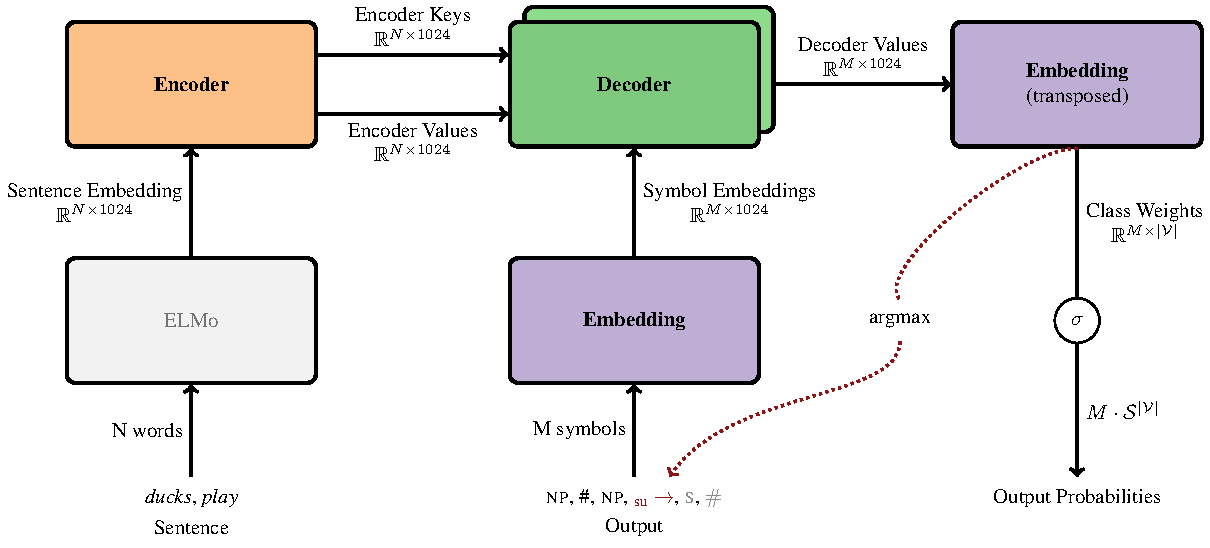
\includegraphics[trim={0mm 0cm 0cm 0cm},clip,scale=1.4]{img/network.pdf}
\end{center}

    
\section{Results}
\vspace{-50pt}
\begin{center}
\begin{tabularx}{0.9\textwidth}{@{}msssss@{}}
\multicolumn{1}{m}{} & \multicolumn{5}{s}{\centering \% Type Accuracy} \\
\cmidrule{2-6}
Model & \fontsizesmall Unseen & \fontsizesmall Rare & \fontsizesmall Medium & \fontsizesmall Common & \fontsizesmall Overall \\
\cmidrule{1-6}
\fontsizesmall Predictive Baseline & -- & 23.9 & 59.0 & 89.9 & 87.2\\
\color{methods}\fontsizesmall \textbf{Constructive} & \textbf{19.2} & \textbf{45.7} & \textbf{65.6} & \textbf{89.9} & \textbf{88.0}\\
\end{tabularx}
\end{center}

\vspace{20pt}
\begin{itemize}
    \item \textbf{Generalization} to rare and unseen types.
    \item Constructed types are {\bf well-formed} --- perfect acquisition of type syntax.
    \item Phrasal \textbf{self-consistency} --- good grasp of sentence/proof structure.
    \item \textbf{Non-trivial} new types but limited over-generation.
\end{itemize}

\vspace{40pt}

\centering{
    \begin{mybox}
    {
        \centering 
        % \includegraphics{img/Unitag_QRCode_1563396899620.png}
        
\includegraphics[scale=0.135]{qr-code.png}
    }
    \end{mybox}
}
}
{
\vfill
\begin{center}
    \vfill
    
    
\includegraphics[scale=0.16]{img/uu.png}
    
    \color{black}Utrecht University
\end{center}
}
{
\vfill
\begin{center}
    \vfill 
    
    
\includegraphics[trim={9cm 5cm 9cm 1cm},clip,scale=0.2]{img/NWO-logo.jpg}
    
    \color{black}Dutch Research 
    
    Council
    
\end{center}\hfill
}
\end{document}
